%% article.tex --- AI4Science-YSDA 2026, English anonymized submission.
%% Build: pdflatex article ; bibtex article ; pdflatex article ; pdflatex article

\documentclass{article}

\usepackage[english]{ai4science_ysda2026}

\usepackage[T1]{fontenc}
\usepackage[utf8]{inputenc}

\usepackage{amsmath}
\usepackage{amssymb}
\usepackage{amsthm}
\usepackage{graphicx}
\usepackage{booktabs}
\usepackage{placeins}

\icmltitlerunning{Frac-Hit Prediction from LF-DAS}

\begin{document}

\twocolumn[
  \icmltitle{Frac-Hit Prediction from LF-DAS:\\
    Physics-Informed Deep Learning with a Traffic-Light Output}

  \begin{icmlauthorlist}
    \icmlauthor{Anonymous Author}{aff}
  \end{icmlauthorlist}

  \icmlaffiliation{aff}{Affiliation hidden for review}
  \icmlcorrespondingauthor{Anonymous Author}{anon@example.org}

  \icmlkeywords{LF-DAS, hydraulic fracturing, frac-hit, ResNet, GRU,
                multiple-instance learning, causal preprocessing,
                formal verification, Lean 4}

  \vskip 0.3in
]

\printAffiliationsAndNotice{}

\begin{abstract}
Live detection of hydraulic-fracture hits (``frac-hits'') in offset
monitoring wells from low-frequency distributed acoustic sensing is
posed as a classification-with-timing problem rather than a regression
over arrival time. On an honest leave-pair-out split the minute-level
time-to-hit falls below the noise floor of the signal --- a constant
that ignores the data beats every learned predictor --- so the deployed
system emits a three-state alarm (green / yellow / red) from a
thresholded probability and uses the classical converging-wedge
kinematics only in the last minutes. The detector is a pretrained
ResNet-18 coupled with a causal GRU over minute embeddings, scanned
across the fibre in overlapping fixed-depth windows (multiple-instance
learning). On a field corpus of 626 stage recordings and 144 manually
built hit labels across eight basins, the deployed model achieves
PR-AUC $0.919$, recall $0.867$ at a false-alarm rate of $0.080$, and a
median lead time of 47\,min. A separate three-layer verification stack
--- schema validator, Hypothesis property tests, and a Lean~4 formal
proof of causal preprocessing --- quantifies the cost of the look-ahead
leak that silently inflated a prior CNN: $+0.448$ phantom AUC
($95\%$~CI $[+0.376, +0.519]$), motivating the strict causal
normalisation used throughout.
\end{abstract}

% ─────────────────────────────────────────────────────────────────────────
\section{Introduction}
\label{sec:intro}

A \emph{frac-hit} is the arrival of a hydraulic fracture at an offset
monitoring well, detected on the strain / strain-rate waterfall of a
low-frequency DAS fibre. Who cares depends on which side of the fence
the operator is on. In infill-stimulation campaigns the hit is a
warning: a producing parent well is being drained or damaged by the
child frac, with ESP damage, water intrusion, and pressure interference
as the operational consequences --- the goal is to detect early and
divert. In EGS and geothermal stimulation the hit is the \emph{target}:
the point of first connection between the stimulated zone and the
production well. In both cases an operator wants, in the next minutes,
one of two signals: ``a hit is approaching'' and, if possible, ``how
soon''.

What makes this hard --- and what shapes the whole paper --- is less
the algorithm and more the data situation. At the start of the project
there was no corpus: hit labels had to be assembled piecemeal, stage by
stage, across whatever datasets could be accessed. The only openly
published field with labels is HFTS-2, and it dominates the corpus
(389~records, 128~hits of the final~144). Training on HFTS alone does
not transfer: the acquisition geometry, the strain magnitudes and the
noise floor are specific to one rock and one interrogator; on
operationally relevant fields (Vineyard, FORGE, Laja/YPF, CrownQuest,
PetroHunt, Vista) the model has to generalise from a handful of
records. Labels themselves are manual --- there is no ground truth ---
and they were built by several engineers over the course of a year, so
a residual label noise is baked in. A physics-based synthetic model was
attempted in parallel and it reproduces the FWHM-collapse of the wedge
qualitatively, but in detail the synthetic signals look very little
like field data (missing low-frequency drift, missing fibre
heterogeneity, idealised source geometry), so it was used only as a
sanity check on preprocessing, not as training data.

The second hard fact is that minute-level arrival time is weakly
observable in this corpus. On a leave-pair-out evaluation, predicting
the median $t_\text{hit}$ of the known well pair beats every learned
regressor; only the classification head carries signal. The deployable
system therefore returns a probabilistic alarm with a coarse
operational surface (traffic light) and refines the ETA with classical
converging-wedge kinematics only in the last minutes. Everything rests
on strict causality of the preprocessing --- and on being able to prove
it. That verification turns out to be what separates the current model
from the previous one it replaced.

% ─────────────────────────────────────────────────────────────────────────
\section{Problem statement}
\label{sec:problem}

\textbf{Given.} A per-stage array $X \in \mathbb{R}^{T \times D}$
sampled at 1\,min after causal low-pass decimation, with
$T \in [10,\,615]$ and $D \in [400,\,3000]$. A labelled set
$\{(X_i, y_i)\}_{i=1}^{N}$, $y_i \in \{0, 1\}$ (hit / no-hit),
$t_{\text{hit}, i}$ for positives. $N = 626$, 144 positives, eight
basins.

\textbf{Goal.} A causal predictor $\hat P_t = f(X_{\le t})$ with
calibrated thresholds such that on a held-out split the operational
requirements hold \emph{per file} (the operator sees one alarm per
recording).

\textbf{Acceptance.} Deploy-faithful evaluation on a 40-file validation
split must reach PR-AUC $\ge 0.90$ and recall $\ge 0.85$ at
FAR $\le 0.10$; preprocessing must be provably causal
(see~\S\ref{sec:verification}).

% ─────────────────────────────────────────────────────────────────────────
\section{Related work}
\label{sec:related}

The physical interpretation of LF-DAS and the converging-wedge
signature are developed in~\cite{liu2020,li2024}; multi-stage
diagnostics with distributed fibre is covered
in~\cite{pakhotina2020,alaamri2024}. Real-time monitoring and
microseismic context are classical~\cite{cipolla2002,lecalvez2007}.
Physics-informed learning for hydraulic fracturing as a generic
framework is treated in~\cite{khan2024piml}. Adjacent work targets
cluster efficiency and early screen-out identification from
high-frequency pressure and DAS~\cite{korkin2020hfpressure,%
korkin2024cluster,alaamri2025oman}, and controlled DAS performance
characterisation~\cite{kuznetsov2025urtec,lecalvez2025integrated,parkhonyuk2018}.
Compared to the above, the present work converts the problem from
regression of arrival time into detection with a traffic-light output,
pins causal preprocessing with a formal proof, and quantifies the cost
of violating it.

% ─────────────────────────────────────────────────────────────────────────
\section{Method}
\label{sec:method}

\textbf{Causal preprocessing.} Per channel, the first $W = 30$ warm-up
minutes supply a robust causal normalisation:
$m = \mathrm{median}(x_{\le W})$,
$s = 1.4826\,\mathrm{MAD}(x_{\le W})$, and
$x_\text{norm} = \mathrm{clip}((x - m)/s,\,-8,\,8)$. A mild depth
smoothing ($\sigma = 1.2$ bins) and a resample to 64 bins follow. The
pipeline consumes only data up to the current minute; the formal proof
of that invariant is in~\S\ref{sec:verification}.

\textbf{Backbone: ResNet-18 + causal GRU.} Each minute is encoded as a
two-channel image
$(2, T_\text{win}, D_\text{ctx}) = (2, 32, 64)$ built from strain and
strain-rate. An ImageNet-pretrained ResNet-18, with BatchNorm replaced
by GroupNorm and its stem rewired to two channels, produces a
$512$-dim embedding per minute. A one-directional GRU with hidden
size~128 consumes the embedding stream in time order and emits two
heads: a Bernoulli hit probability $P(\text{hit})$ and a regression
head $(\mu, \log\sigma)$ for the remaining-time estimate. ImageNet
pretraining is used because the corpus is small; abandoning it in
favour of a bespoke CNN loses both PR-AUC and sample efficiency.

\textbf{Multiple-instance scan.} Rather than one network per recording,
the same network is applied in fixed-size depth windows of $128$\,m
with a $64$\,m stride (50\% overlap); the window length and stride are
read from the deployed checkpoint. File-level probability is the max
over windows; the per-depth location is the window of the maximum.
This keeps the same operator across different fibre geometries and
discourages memorising per-field band placement.

\textbf{Traffic light.} Rather than minutes, the UI shows one of three
colours. Red is non-latching with a 1\,min hold and requires
$\text{persist} = 3$ consecutive minutes above
$\mathrm{thr}_\text{red} = 0.199$; yellow is instantaneous and uses
$\mathrm{thr}_\text{yel} = 0.115$. Thresholds are tied to the deployed
checkpoint and selected on tolerated FAR \emph{per file}. In the last
few minutes, when the classical FWHM wedge extrapolation becomes
accurate~\cite{liu2020,li2024}, it supplies a refined ETA, gated to
fire only when it itself promises a short remaining time.

% ─────────────────────────────────────────────────────────────────────────
\section{Verification}
\label{sec:verification}

Because look-ahead leakage in per-file normalisation once produced
excellent but unreproducible metrics, the deployed pipeline is
protected by three independent layers.

\emph{Schema validator} --- every \texttt{.npz} record is checked for
required keys, shape consistency, finite values, monotone depth, and
label consistency. On the current corpus: $626/626$ pass, with
warnings only for known heterogeneities (mixed interrogator units; one
\texttt{label\_D\_mismatch} flagged for manual review).

\emph{Property tests (Hypothesis).} The guard invariant is that
output~$i$ depends only on input up to $i \cdot R$. Perturbing the
input from index~$k$ onwards must leave the first
$\lfloor (k-1)/R \rfloor + 1$ output rows bitwise unchanged.
Twenty randomised tests pass in 2.3\,s.

\emph{Formal proof (Lean~4).} Four theorems close the invariant for
\emph{all} inputs rather than a random sample:
\texttt{bdiff\_causal}, \texttt{ewma\_causal}, \texttt{P\_causal} (the
full composition) and \texttt{P\_zero}. The SciLib checker reports
\texttt{success:\,true} with zero \texttt{sorry}, \texttt{admit}, or
added \texttt{axiom}.

\emph{Numerical cost of the leak.} A controlled five-seed experiment
compares two otherwise identical classifiers on an early-window
feature of a synthetic frac-hit dataset: one uses the causal
normalisation above, the other normalises by whole-sequence
statistics. The acceptance rule --- declared before any number was
produced --- requires the paired
$\Delta = \mathrm{AUC}_\text{leaky} - \mathrm{AUC}_\text{causal}$ to
have a $95\%$ CI excluding zero, $|\Delta| > 0.05$, and a
Holm-corrected paired $t$ with $p < 0.05$. All three hold:
$\Delta = +0.448$, $95\%$~CI $[+0.376, +0.519]$, $d_z = 7.76$,
$p_\text{Holm} = 10^{-4}$. A one-line patch replacing backward
difference with centred difference in \texttt{strain\_rate\_causal}
is caught by property test
\texttt{test\_strain\_rate\_causal\_no\_future\_leak}:
2~failed / 12~passed before the fix, 14~passed after.

% ─────────────────────────────────────────────────────────────────────────
\section{Experiment}
\label{sec:experiment}

Deploy-faithful evaluation is carried out on a held-out 40-file
validation split of the ResNet checkpoint; multi-horizon calibration
(ECE $<5\%$ on horizons up to 40\,min) is verified in parallel.

\begin{table}[t]
  \caption{Deploy-faithful evaluation on a 40-file validation split:
    ResNet-18 + GRU + MIL against the previous MIL architecture.}
  \label{tab:res}
  \centering
  \small
  \setlength{\tabcolsep}{3.5pt}
  \begin{tabular}{@{}lcccc@{}}
    \toprule
    Model & Recall & FAR & PR-AUC & DC \\
    \midrule
    Windowed MIL (previous) & 0.824 & 0.087 & 0.885 & 0.216 \\
    \textbf{ResNet + GRU}   & \textbf{0.867} & \textbf{0.080}
                            & \textbf{0.919} & \textbf{0.133} \\
    \bottomrule
  \end{tabular}
\end{table}

On the full corpus (626 files, threshold calibration) the deployed
operating point reaches recall $0.812$, FAR $0.041$ and median lead
time $47$\,min.

Figure~\ref{fig:forge} shows a clean FORGE stage~\cite{kuznetsov2026utahforge}:
the converging wedge is unambiguous on the strain-rate waterfall, the
alarm fires well before the event, the 3D view highlights the active
depth window, and the classical ETA pulls in during the last few
minutes. Figure~\ref{fig:twohump} is the small but useful piece of
evidence that scanning in depth is doing real work: on an HFTS-2
stage labelled with a single hit, the per-window $P(\text{hit})$ peaks
twice. Reinspection of the waterfall confirmed the second peak is a
real event, missed at labelling time.

\begin{figure}[t]
  \centering
  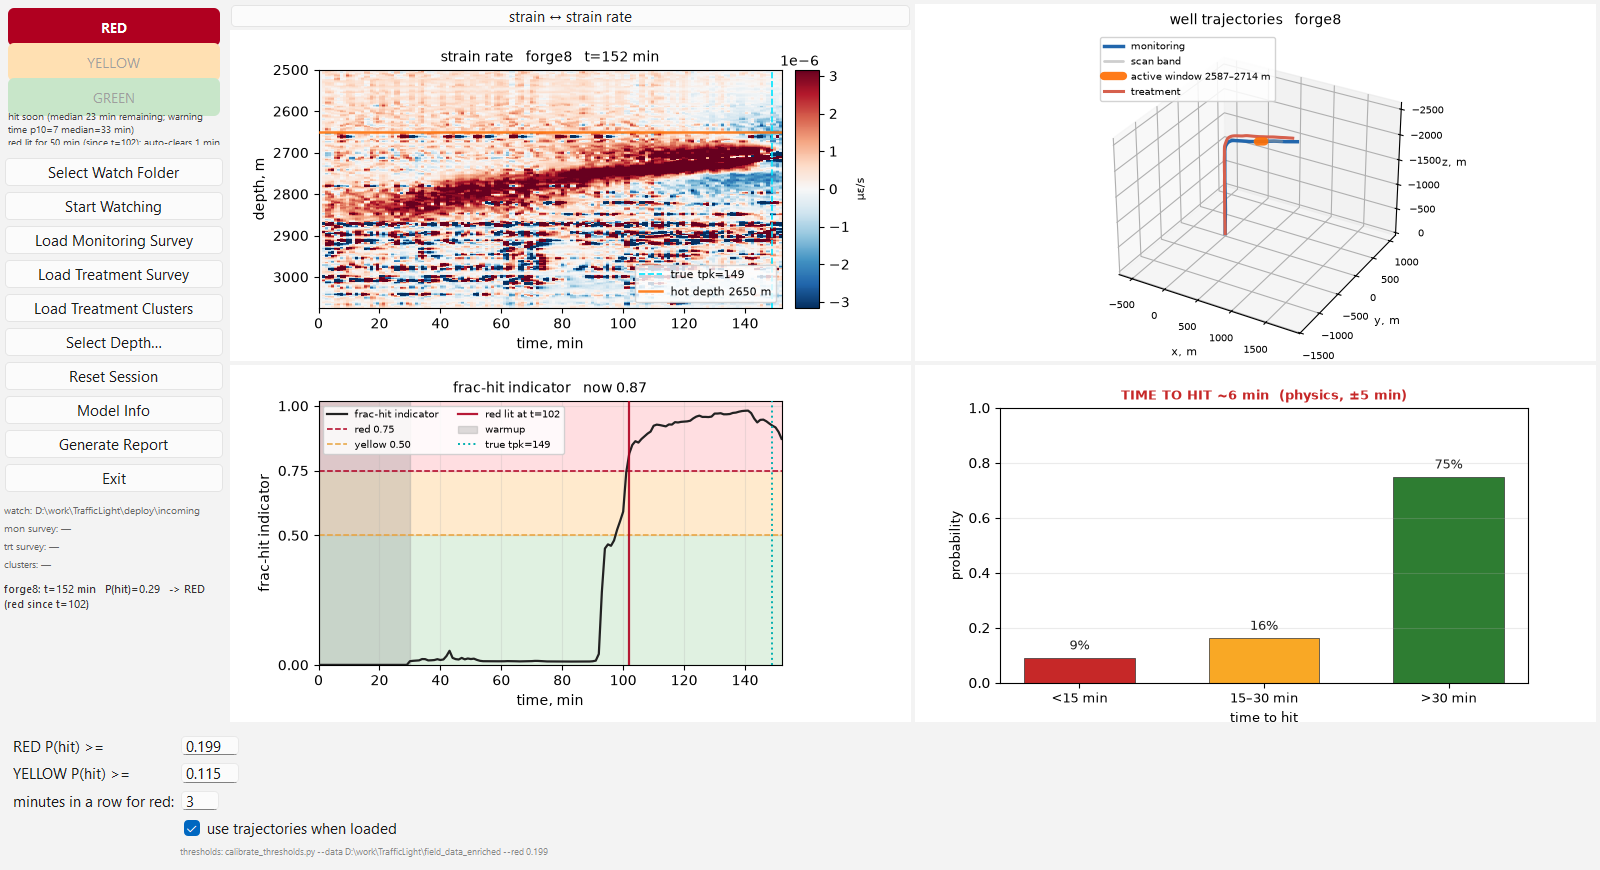
\includegraphics[width=\columnwidth]{figs/forge8_2.png}
  \caption{A clean FORGE stage, live. The strain-rate waterfall
    (top-right) shows the converging wedge; $P(\text{hit})$ saturates
    minutes before the event; the traffic light turns red
    (non-latching, 1\,min hold); the 3D view highlights the active
    depth window.}
  \label{fig:forge}
\end{figure}

\begin{figure}[t]
  \centering
  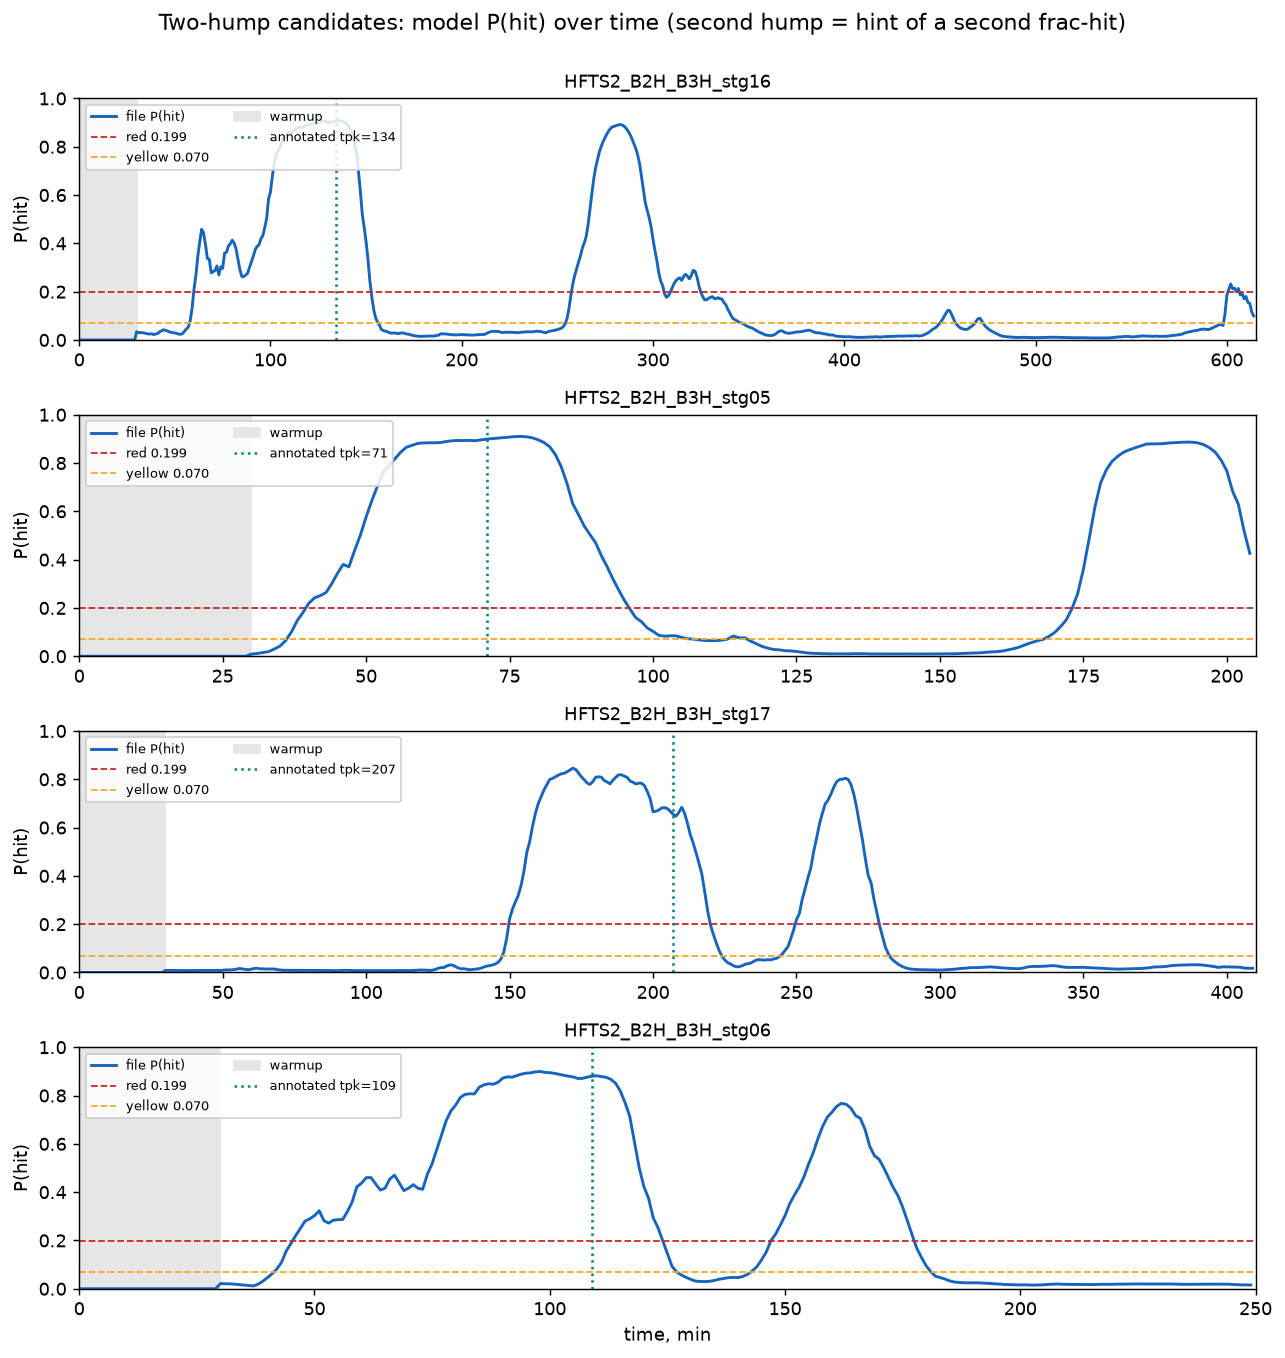
\includegraphics[width=0.85\columnwidth]{figs/twohump_Phit.png}
  \caption{File-level $P(\text{hit})$ over time on an HFTS-2 stage
    labelled with a single hit (dashed green). The windowed MIL scan
    returns two clearly separated peaks; the second one, previously
    unlabelled, is a real event confirmed on reinspection of the
    waterfall.}
  \label{fig:twohump}
\end{figure}

% ─────────────────────────────────────────────────────────────────────────
\section{Limitations}
\label{sec:limitations}

Three caveats sit in the numbers. First, the effective sample size is
the number of independent well pairs, not records --- per-pair
$t_\text{hit}$ medians (65, 70, 108, 179\,min) explain most of what
the time head learned, which is why the system is reported as a
detector. Second, the ResNet recipe (G2, no-bucket) was fixed by
multi-fold search on the same corpus that supplies the operating
point; an unconditional leave-one-field-out would widen both sides of
the Pareto front. Third, on sparser fields (Vineyard, CrownQuest) the
signal is often visible to the eye but activation maps drift off the
deformation core, suggesting the backbone has not seen enough of that
kind of rock. The guarantees in~\S\ref{sec:verification} cover
preprocessing only (backward difference, EWMA, causal decimation); the
GRU warm-up and the MIL pooling stay inside the empirical envelope.

Two further pieces of context. Labels are manual and were authored by
several engineers; the resulting label noise is not modelled, which
likely inflates the apparent FAR on ambiguous records. A physics-based
synthetic generator was tried as a training-augmentation source and
discarded: the synthetic waterfalls match the FWHM-collapse of the
wedge qualitatively but miss the low-frequency drift, the fibre
heterogeneity and the acquisition noise floor of the field data, so
models trained on synthetic transfer poorly.

% ─────────────────────────────────────────────────────────────────────────
\section{Reproducibility}
\label{sec:reproducibility}

Source code and data for the verification stack live at
\anonymized{\url{https://github.com/REDACTED/ai4science/tree/article}}.
The git tag is \texttt{article/41e6861}. Environment:
Python~3.11, NumPy~1.26, PyTorch~2.3, scikit-learn~1.5,
Lean~4 with SciLib. Table~\ref{tab:res} and
Figures~\ref{fig:forge},~\ref{fig:twohump} are drawn from the project
deployment report; the numerical leak cost is obtained with
\texttt{python -m pytest -q checks} (five seeds,
see \texttt{checks/experiment.py}).

% ─────────────────────────────────────────────────────────────────────────
\section{Conclusion}
\label{sec:conclusion}

A frac-hit detector that pairs an ImageNet-pretrained ResNet-18 with a
causal GRU and a windowed MIL scan is competitive on a small,
heterogeneous field corpus: PR-AUC $0.919$, recall $0.867$ at FAR
$0.080$, median lead time $47$\,min. The operational surface is
intentionally coarse --- a three-state traffic light --- because
minute-level timing is provably not in the signal at this corpus size.
Causal preprocessing is formalised in Lean~4 and empirically shown to
be worth $+0.45$ AUC if violated. Next steps: an honest
leave-one-field-out of the ResNet recipe, more data on sparse fields,
and a formal treatment of the GRU warm-up.

\begin{aiusage}[Fragments generated by a model or taken from sources,
  and how each was verified.]
  \texttt{src/preprocess.py},
  \texttt{src/wedge\_near.py}
    & \written{} & --- & property tests + Lean \\
  \texttt{checks/test\_*.py},
  \texttt{validate\_data.py}
    & \generated{} & Goose; Cursor (Claude)
    & \texttt{pytest -q checks}; non-vacuous asserts \\
  \texttt{checks/experiment.py} (leak cost)
    & \generated{} & Cursor (Claude)
    & five-seed run; acceptance rule declared ex ante \\
  \texttt{checks/CausalPreprocess.lean}
    & \generated{} & Goose draft + author edits
    & SciLib \texttt{lean\_check success:true}, 0~\texttt{sorry} \\
  \S\ref{sec:intro}--\S\ref{sec:conclusion} of this paper
    & \written{} & --- (light polish by Cursor)
    & numbers cross-checked against
      \texttt{checks/results/} \\
  Figures~\ref{fig:forge},~\ref{fig:twohump}
    & \sourced{} & project materials
    & visual comparison with originals \\
\end{aiusage}

\acknowledgements{The author thanks project colleagues for the LF-DAS
field corpus and internal review, and the AI4Science course staff for
comments on the problem statement.}

\bibliography{refs}
\bibliographystyle{ai4science_ysda2026}

\end{document}
